\documentclass[]{article}
\usepackage{lmodern}
\usepackage{amssymb,amsmath}
\usepackage{ifxetex,ifluatex}
\usepackage{fixltx2e} % provides \textsubscript
\ifnum 0\ifxetex 1\fi\ifluatex 1\fi=0 % if pdftex
  \usepackage[T1]{fontenc}
  \usepackage[utf8]{inputenc}
\else % if luatex or xelatex
  \ifxetex
    \usepackage{mathspec}
  \else
    \usepackage{fontspec}
  \fi
  \defaultfontfeatures{Ligatures=TeX,Scale=MatchLowercase}
\fi
% use upquote if available, for straight quotes in verbatim environments
\IfFileExists{upquote.sty}{\usepackage{upquote}}{}
% use microtype if available
\IfFileExists{microtype.sty}{%
\usepackage{microtype}
\UseMicrotypeSet[protrusion]{basicmath} % disable protrusion for tt fonts
}{}
\usepackage[margin=1in]{geometry}
\usepackage{hyperref}
\hypersetup{unicode=true,
            pdfborder={0 0 0},
            breaklinks=true}
\urlstyle{same}  % don't use monospace font for urls
\usepackage{graphicx,grffile}
\makeatletter
\def\maxwidth{\ifdim\Gin@nat@width>\linewidth\linewidth\else\Gin@nat@width\fi}
\def\maxheight{\ifdim\Gin@nat@height>\textheight\textheight\else\Gin@nat@height\fi}
\makeatother
% Scale images if necessary, so that they will not overflow the page
% margins by default, and it is still possible to overwrite the defaults
% using explicit options in \includegraphics[width, height, ...]{}
\setkeys{Gin}{width=\maxwidth,height=\maxheight,keepaspectratio}
\IfFileExists{parskip.sty}{%
\usepackage{parskip}
}{% else
\setlength{\parindent}{0pt}
\setlength{\parskip}{6pt plus 2pt minus 1pt}
}
\setlength{\emergencystretch}{3em}  % prevent overfull lines
\providecommand{\tightlist}{%
  \setlength{\itemsep}{0pt}\setlength{\parskip}{0pt}}
\setcounter{secnumdepth}{0}
% Redefines (sub)paragraphs to behave more like sections
\ifx\paragraph\undefined\else
\let\oldparagraph\paragraph
\renewcommand{\paragraph}[1]{\oldparagraph{#1}\mbox{}}
\fi
\ifx\subparagraph\undefined\else
\let\oldsubparagraph\subparagraph
\renewcommand{\subparagraph}[1]{\oldsubparagraph{#1}\mbox{}}
\fi

%%% Use protect on footnotes to avoid problems with footnotes in titles
\let\rmarkdownfootnote\footnote%
\def\footnote{\protect\rmarkdownfootnote}

%%% Change title format to be more compact
\usepackage{titling}

% Create subtitle command for use in maketitle
\newcommand{\subtitle}[1]{
  \posttitle{
    \begin{center}\large#1\end{center}
    }
}

\setlength{\droptitle}{-2em}

  \title{}
    \pretitle{\vspace{\droptitle}}
  \posttitle{}
    \author{}
    \preauthor{}\postauthor{}
    \date{}
    \predate{}\postdate{}
  
\usepackage{float}

\begin{document}

\begin{centering}

\vspace*{5 cm}

\Huge

{\bf Administración e Instalación de Linux CentOS (Windows 10)}

\vspace{3 cm}

\Large
Marco Andrés Vázquez Hernández

\vspace{1 cm}
\normalsize
Práctica 1: Documentación. 

Agosto de 2018

\normalsize
Instituto Politécnico Nacional


\end{centering}

\newpage

\section{Prerequisitos (Virtual)}\label{prerequisitos-virtual}

\subsection{Instalación de Virtual Box (Windows
10)}\label{instalacion-de-virtual-box-windows-10}

Descargar la última versión de Virtual Box:
\url{https://virtualbox/wiki/Downloads}.

\subsection{Instalación de Vagrant (Windows
10)}\label{instalacion-de-vagrant-windows-10}

Descargar la última versión de Vagrant:
\url{https://vagrantup.com/downloads.html}.

\subsection{Uso de Tools-CIC}\label{uso-de-tools-cic}

Ejecutar desde la terminal (Powershell):

\begin{verbatim}
mkdir ~/Prac
cd ~/Prac
vagrant init nogala/centos --box-version 1
vagrant plugin install vagrant-vbguest
vagrant up
vagrant ssh
\end{verbatim}

Nota: Hacer update y upgrade

\begin{verbatim}
sudo yum update
sudo yum upgrade
\end{verbatim}

\section{1) Cambio de nombre del host}\label{cambio-de-nombre-del-host}

\begin{verbatim}
sudo hostnamectl set-hostname vazquez
\end{verbatim}

Para que el cambio tenga efecto se necesita reiniciar.

\begin{figure}[htbp]
\centering
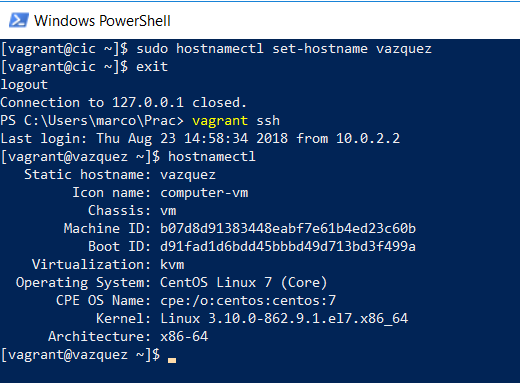
\includegraphics{hostnamectl.png}
\end{figure}

\section{2) Actualización y sincronización de la hora y fecha con
servicio
NTP}\label{actualizacion-y-sincronizacion-de-la-hora-y-fecha-con-servicio-ntp}

Para cambiar la hora se puede elegir de una lista:

\begin{verbatim}
timedatectl list-timezones
timedatectl set-timezone America/Mexico_City
hwclock --systohc
\end{verbatim}

Para el servicio NTP se instalará chronyd

\begin{verbatim}
yum install -y chronyd
\end{verbatim}

Se cambia el archivo /etc/chrony.conf con\\
server 0.mx.pool.ntp.org\\
server 1.north-america.pool.ntp.org\\
server 2.north-america.pool.ntp.org

\begin{verbatim}
nano /etc/chrony.conf
systemctl start chronyd
systemctl enable chronyd
\end{verbatim}

Para verificar que se está funcionando correctamente y las fuentes que
se están usando ejecutar:

\begin{verbatim}
timedatectl
chronyc sources 
\end{verbatim}

\begin{figure}[htbp]
\centering
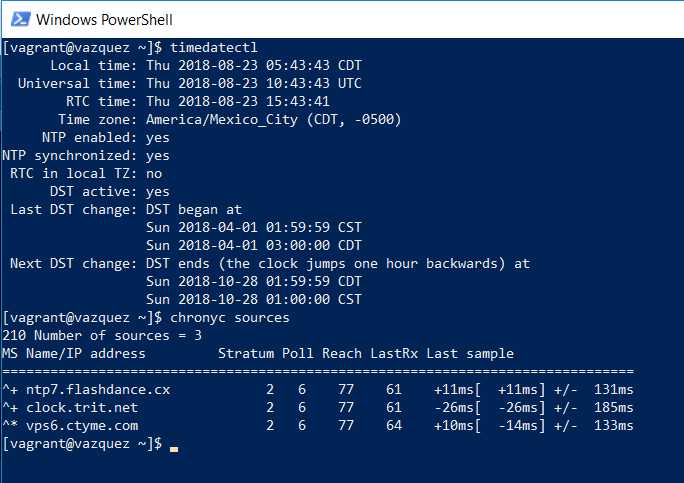
\includegraphics{NTP.png}
\end{figure}

\section{3.a) Instalación de Java}\label{a-instalacion-de-java}

Se revisa la versión más reciente de Java desde el navegador y se
realiza un wget (si no se tiene wget se instala):

\begin{verbatim}
yum install wget
wget --no-cookies --no-check-certificate --header "Cookie:
gpw_e24=http%3A%2F%2Fwww.oracle.com%2F; oraclelicense=accept-securebackup-cookie"
"http://download.oracle.com/otn-pub/java/jdk/8u181-b13/96a7b8442fe848ef90c96a2fad6ed6d1/
jdk-8u181-linux-x64.rpm"
\end{verbatim}

Se instala localmente desde la carpeta en donde lo descargamos:

\begin{verbatim}
yum localinstall -y jdk-8u181-linux-x64.rpm
\end{verbatim}

Revisar y cambiar a la última versión de java con los comandos:

\begin{verbatim}
cd /usr/java
ll
alternatives --config java
\end{verbatim}

Crear la variable de entorno HOME\_JAVA (como root)

\begin{verbatim}
echo "export JAVA_HOME=/usr/java/latest" >> /etc/environment
\end{verbatim}

Para revisar que la instalación haya sido correcta:

\begin{verbatim}
java -version
echo $JAVA_HOME
\end{verbatim}

\begin{figure}[htbp]
\centering
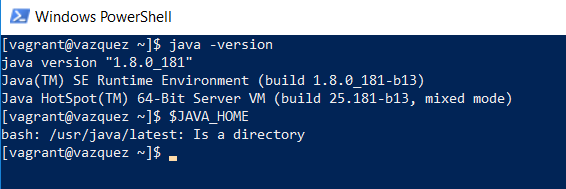
\includegraphics{java.png}
\end{figure}

\section{3.b) Instalación de Maven}\label{b-instalacion-de-maven}

Ejecutar los comandos:

\begin{verbatim}
yum install yum-utils -y
sudo yum install yum-utils -y
sudo yum groupinstall "Development Tools" -y
cd /usr/local/src
wget http://www-eu.apache.org/dist/maven/maven-3/3.5.4/binaries/apache-maven-3.5.4-bin.tar.gz
tar -xvzf apache-maven-3.5.4-bin.tar.gz 
rm apache-maven-3.5.4-bin.tar.gz 
mv apache-maven-3.5.4 apache-maven
\end{verbatim}

Para cambiar los paths, crear un archivo en /etc/profile.d con nombre
maven.sh que contenga lo siguiente:

\begin{verbatim}
cd /etc/profile.d/
nano maven.sh
\end{verbatim}

\begin{verbatim}
# Apache Maven Environment Variables  
# MAVEN_HOME for Maven 1 - M2_HOME for Maven 2  
export M2_HOME=/usr/local/src/apache-maven
export PATH=${M2_HOME}/bin:${PATH}
\end{verbatim}

Permitir la ejecución de tal archivo con:

\begin{verbatim}
sudo chmod +x maven.sh
\end{verbatim}

Para revisar que este instalado correctamente ejecutar:

\begin{verbatim}
mvn --version
\end{verbatim}

\begin{figure}[htbp]
\centering
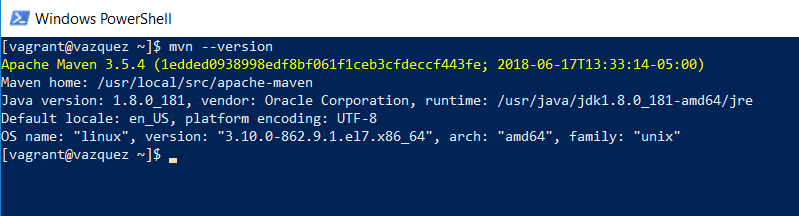
\includegraphics{maven.png}
\end{figure}

\section{3.c) Instalación de Python (Desde Código
Fuente)}\label{c-instalacion-de-python-desde-codigo-fuente}

Instalar prerequisitos:

\begin{verbatim}
sudo yum install gcc openssl-devel bzip2-devel libffi-devel -y
\end{verbatim}

Buscar en internet la última versión de Python (Gzipped source tarball)
y extraer en /usr/local/src

\begin{verbatim}
cd /usr/local/src/
sudo wget https://www.python.org/ftp/python/3.7.0/Python-3.7.0.tgz
sudo tar xvzf Python-3.7.0.tgz
\end{verbatim}

Entrar en la carpeta y configurar con los siguientes comandos

\begin{verbatim}
cd Python-3.7.0/
sudo ./configure
sudo make
sudo make install
\end{verbatim}

Para verificar que está instalado:

\begin{verbatim}
python3 --version
\end{verbatim}

\begin{figure}[htbp]
\centering
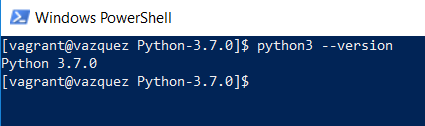
\includegraphics{python.png}
\end{figure}

\section{4) Configuración de las herramientas de rendimiento y
administración del sistema (tmux, htop,
git)}\label{configuracion-de-las-herramientas-de-rendimiento-y-administracion-del-sistema-tmux-htop-git}

Para instalar tmux:

\begin{verbatim}
sudo yum install epel-release
sudo yum install tmux
\end{verbatim}

para instalar htop:

\begin{verbatim}
wget dl.fedoraproject.org/pub/epel/7/x86_64/Packages/e/epel-release-7-11.noarch.rpm
sudo rpm -ihv epel-release-7-11.noarch.rpm 
sudo yum install htop
\end{verbatim}

Para git se recomienda crear otro (super)usuario:

\begin{verbatim}
sudo useradd marco
sudo usermod -G wheel marco
sudo passwd marco
su marco
\end{verbatim}

Para instalar git y configurar el usuario:

\begin{verbatim}
sudo yum install git -y
sudo git config --global user.name "MARCOVH"
sudo git config --global user.email "marcovazquezh@gmail.com"
sudo git config --list
\end{verbatim}

Para crear un nuevo repositorio crearlo en la cuenta en github.com:

\begin{figure}[htbp]
\centering
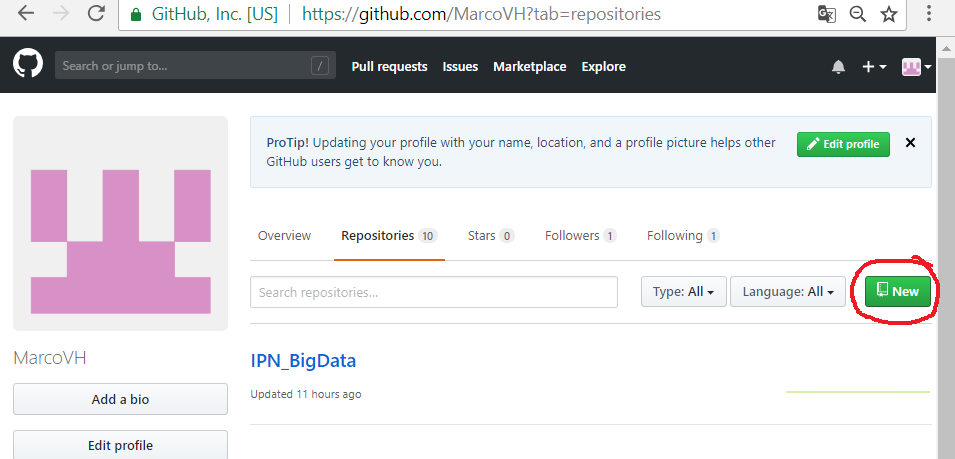
\includegraphics{github.png}
\end{figure}

Crear la carpeta en la maquina junto con un archivo README.md y
configurarlo para git con commit y push.

\begin{verbatim}
sudo mkdir Practica-1
cd Practica-1
sudo nano README.md
sudo git init
sudo git add README.md
sudo git commit -m "primer commit"
sudo git remote add origin https://github.com/MarcoVH/Practica-1.git
sudo git push -u origin master
\end{verbatim}

Si todo es correcto la pantalla mostrará:

\begin{figure}[htbp]
\centering
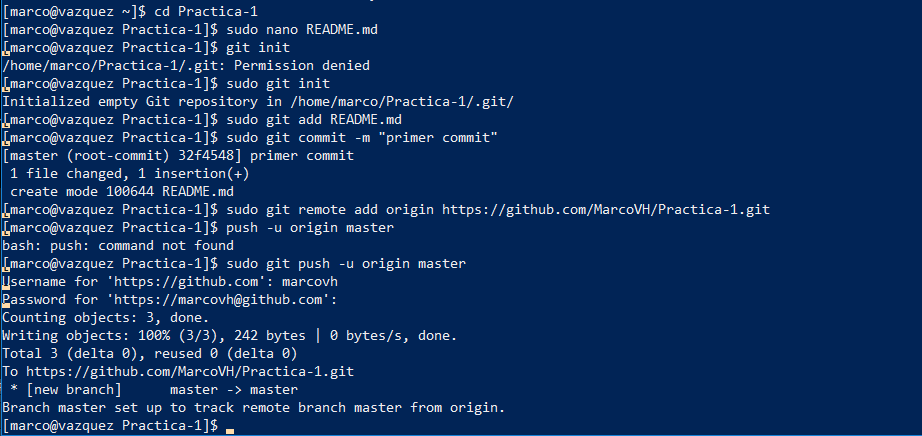
\includegraphics{git.png}
\end{figure}

Y el repositorio en github tendrá el README.md

\section{5) Instalación y configuración del servidor de web
(httpd)}\label{instalacion-y-configuracion-del-servidor-de-web-httpd}

NOTA: Para que funcione con vagrant, el archivo Vagrantfile debe de
tener la línea ``config.vm.network''forwarded\_port``, guest: 80, host:
8080'' no comentada.

Para instalar httpd

\begin{verbatim}
sudo yum install httpd
sudo service httpd start
\end{verbatim}

Para checar que esté funcionando correctamente se ejecuta

\begin{verbatim}
sudo service httpd status
\end{verbatim}

También tiene que aparecer la página de prueba de Apache HTTP server
poniendo en el navegador localhost:8080 (de acuerdo al puerto que se
configure en el Vagrantfile para virtualizaciones):

\begin{figure}[htbp]
\centering
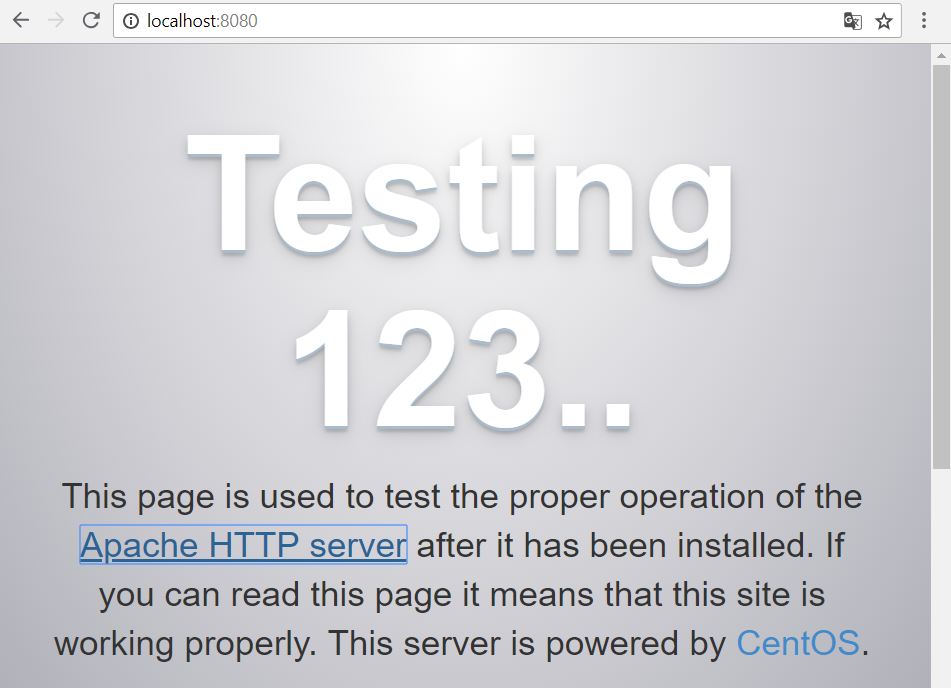
\includegraphics{httpd.png}
\end{figure}


\end{document}
